\chapter{Main Rapture concepts}

The API section of this document gives a more thorough treatment to each of the major concepts in \Rapture. This section
presents a general overview of the major themes. Nearly every concept in \Rapture and the entities that describe it are
referenced using a uri naming scheme. The following sections describe these concepts.

\section{Data}
One of the prime uses of \Rapture is to manage access to data. \Rapture has the concept of a \emph{repository} which is a
reference to either a data store managed by \Rapture (the data is only updated by \Rapture applications) or
the data is externally managed and \Rapture is simply accessing it "remotely".

Repositories in \Rapture are divided into types.

\subsection{Document Data}
Document data repositories manage data as key/value pairs. The key in \Rapture is a document uri and the value
is typically (but not necessarily) a JSON formatted document. As an example, an abstract view of a document repository would map the following:

\begin{Verbatim}
	doc://test/one/two/three

	{
	  "field" : "value",
		"one" : 1,
		"array" : [ 1, 2, 3, 4]
		"inner" : {
			"a" : 0,
			"b" : 1,
			"c" : true
		}
	}
\end{Verbatim}

The first part of a document uri (\Verb+test+ in the above example) is a reference to a
document repository which is defined by calling the \Rapture API call "createDocRepo". A
document repository in \Rapture is hosted on an underlying database such as MongoDB or Cassandra
and can be versioned. Each document can have metadata associated with it - some information maintained
directly by \Rapture (such as write time, write user) and some information managed directly by
an application.

You can also append on a version qualifier to the end of a document uri. This gives an application
developer the ability to reference absolutely a piece of content in \Rapture that is invariant.

Documents in \Rapture that are formatted as JSON documents work well with the \Reflex scripting language. When
you load a document from \Rapture into \Reflex it is automatically converted into a special "map of maps" structure
which is easily accessible in the scripting language. As an example consider the code below:

\begin{lstlisting}[caption={Reflex document example}, language=reflex]
  doc <-- "//test/one/two/three";
	assert(doc.one == 1);
	doc.one = 2;
	doc --> "//test/one/two/three";
\end{lstlisting}

This example takes the example document above, tests the value of the "one" field and then
changes it to the value of 2. It then writes that document back to \Rapture, which will create a new
version of that document.

\subsection{Series data}

Series data embraces the concept where instead of having a single document (or data value) at a given
uri you would prefer to reference a whole set of documents each indexed with a unique "column" key. If those
keys represent points in time (perhaps "20160101") then the series could represent time series data.

Series repositories are used to manage this particular type of data. Such data could be represented in a document
repository - the uri for the document could include the point in time or the column key. A series repository is simply
much more efficient at storing and accessing this type of data and special API calls are available to return sub-parts of
the series.

The content stored in an individual point of a series can contain any arbitary value type. Typically the value will be
numeric but strings or more complex structures (such as JSON formatted documents) are also supported.

\begin{figure}[htb]
\centering
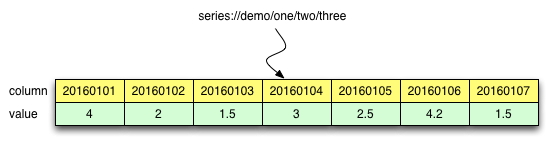
\includegraphics[scale=0.7]{Graphics/SeriesExplain}
\caption{Rapture Series Structure}
\label{fig:RaptureSeriesStructure}
\end{figure}

Figure~\vref{fig:RaptureSeriesStructure} shows the association between a series uri in \Rapture and the data
it "points" to.

\subsection{Blob Data}

Blob (Binary Large OBject) data is used in \Rapture to store data that has some structure or value to an
external application but has no real "meaning" internally to \Rapture. The uri reference to a blob in \Rapture
points to a sequence of bytes -- \Rapture understands (and maintains) the mime-type of the data and its length
and other attributes such as the last writer and write time but it is really just an arbitary store of information.

\Rapture applications tend to use Blob repositories to store spreadsheets, cvs files, images, application code and the like.

\begin{figure}[htb]
\centering
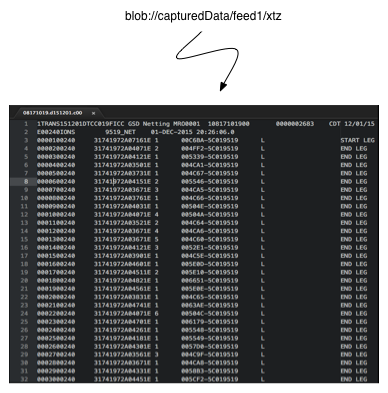
\includegraphics[scale=0.75]{Graphics/RaptureBlobExplain}
\caption{Rapture Blob Structure}
\label{fig:RaptureBlobStructure}
\end{figure}

Figure~\vref{fig:RaptureBlobStructure} shows an example blob uri pointing to a csv file
used in an import/processing application.

\subsection{Structured Data}

Structured data is an alias for "relational data". Structured repositories (equivalent to databases and tables in
a relational database) are used in two completely different ways.

\subsubsection{Internal Structured Data}

A structured data repository can be used internally within an application to store information that is relational in
layout -- the internal reference implies that applications only modify and access this information through the \Rapture API. With
this restriction \Rapture can manage server side caching of the information and propogate changes in a distributed manner to
other servers in a \Rapture environment.

\subsubsection{External Structured Data}

An external structured data repository is simply a well described connection to an external database (and table set). The idea
is that applications and process that are using other \Rapture facilities (the other data types described here, workflows etc.) can
treat this type of external data in the same manner and have a single mechanism for accessing and joining these disparate data sets. In addition
the entitlements system of \Rapture can be used to control access to such a resource.

\section{Workflows}

With data under control with a consistent access mechanism and naming conventions there is often a need in an enterprise application to
manipulate and transform this data in consistent ways. Programs that manipulate data (or do other tasks) can often be broken down into a set of steps
and a workflow in \Rapture is a vehicle for managing the execution of those steps in a controlled and distributed manner.

A sample workflow in \Rapture is shown in Figure~\vref{fig:WorkflowExample}.

\begin{figure}[H]
\centering
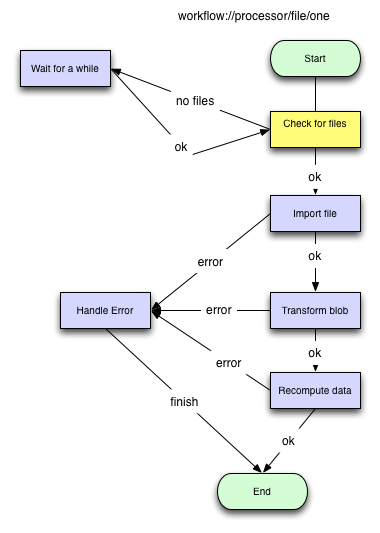
\includegraphics[scale=0.75]{Graphics/RaptureWorkflowExplain}
\caption{Rapture Workflow}
\label{fig:WorkflowExample}
\end{figure}

This workflow, with the unique reference "workflow://processor/file/one" begins at the start step. The first
task (or step) that is executed is "Check for Files". The implementation of a step in a \Rapture workflow can be either
a piece of Java code that is embedded in the \Rapture server (as shown as a workflow extension in Figure~\vref{fig:RaptureExtensionPoints})
or can be a \Reflex script hosted on \Rapture itself. After doing its work the step execution code returns a status code - a piece of text
that is used to point to the next step that will be executed. In this case returning "ok" will move it to the "import file" step and returning
"no files" can point it to the "wait for a while" step. These steps execute in a similar way and the workflow execution continues until we
reach the "End" point.

In a real workflow the "Wait for a while" step would ultimately error out after an extended time.

Workflow steps are associated with server groups and any server in a group can be used to process that step. In this example the yellow first step
needs to run on a special server that has access to a specific file location - once the file(s) are located they are imported into a \Rapture blob repository
and the other steps can run on any server in the environment. This technique and approach allows \Rapture workflows to be distributed across a compute fabric while
still maintaining some constraints on execution.

Workflows can be started (run) using the \Rapture API (see the Decision API later on in this document) or attached to events or schedules.

\section{Scripts}

Scripts in \Rapture refer to programs written in the \Reflex scripting language. That language is described later on in this document.

Scripts have unique references (uris) in \Rapture and can be used in many different ways. Some of the typical use cases are enumerated below:

\begin{itemize}
	\item{Workflow steps can use scripts as part of their execution.}
	\item{Scripts can be run one-off as mini-programs through the \Rapture API.}
	\item{Scripts can be run upon an event firing.}
	\item{Scripts can be executed as part of an AJAX call to a service -- usually returning JSON data controlled by parameters passed in the service call.}
\end{itemize}

\section{Pipelines and Messages}
\Rapture can be a multi-server environment. Coordination is needed between individual servers and this is accomplished through messaging. These messages are
used to coordinate workflow activity or the initiation of any asynchronous style activity. \Rapture abstracts the concept of messaging and message queues from their
implementation. The \Rapture kernel requires at least one of these "pipelines" to be setup for a system to run. In a single server environment
this could be an in memory (in process) implementation - in a multi-server environment the open source RabbitMQ implementation is recommended.

Figure~\vref{fig:PipelineExample} shows the different types of pipeline that could exist in a \Rapture environment.

\begin{figure}[H]
\centering
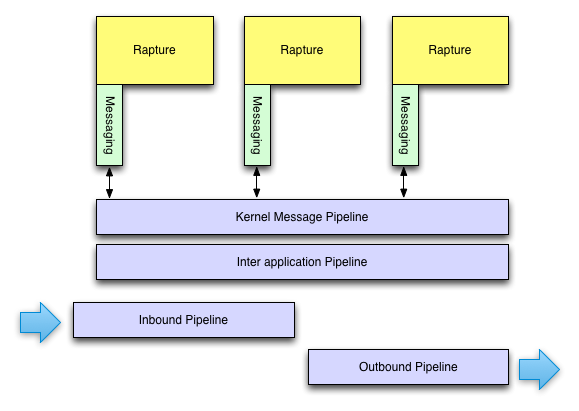
\includegraphics[scale=0.75]{Graphics/PipelineExplain}
\caption{Rapture Pipeline}
\label{fig:PipelineExample}
\end{figure}

The same pipeline system can be used by applications as well. Applications create queues on exchanges and can be both a publisher and a consumer of custom messages
sent on those queues. Some queues could have no endpoint within \Rapture -- they could imply connectivity to external applications and systems. Conversely such queues could
represent inbound queues from external systems. This abstraction separates the application code (the publisher and consumer) from the actual implementation of the transport.

\section{Full Text Search}
Document centric data stores often suffer from the problem that unless you know what you are looking for it can be difficult to
find data in the system. If the only way of finding information was through the URI naming scheme the onus is on the designer
of the naming scheme to properly classify data so it can be found.

To combat this \Rapture supports the use of Full Text Search databases to create secondary indices on the data stored in
document repositories. If so configured, every change and update to document data can also be fed to a full text search engine
and then searches of that engine can be performed to return back the URIs of data that match the search. Full text search queries can
be free in their syntax but (as an example) constructing a query that returns the results of questions such as "find all trades for today in USD that Joe executed with this broker" can
easily be made.

\subsection{Search Repository}
Search is implemented using the same abstraction approach that \Rapture adopts. In the first instance an environment needs to define
one or more "search repositories". A search repository is a mapping from a \Rapture search space to an underyling implementation. The
only implementation supported at present uses Elastic Search as its store.

\subsection{Document Repository Mapping}
Next there needs to be a mapping between a document repository in \Rapture and its associated search repository. Also associated with
this mapping is whether the repository should be indexed at all. If a document repository is mapping the operations such as
put, delete and drop are also cascaded to the appropriate search repository. For convenience there are also API calls to rebuild a search
index if such a mapping is made \emph{after} data has been added to the document repository.

All updates to the search repository are made asynchronously using the internal pipeline feature. This way updates to the index can be
made by background servers in a \Rapture environment instead of just by the server that handled the document API call.

\subsection{Indexes}
\Rapture creates three specific indices in a search repository. Often when querying a search repository the caller can run the query on
all three indices at the same time, or they can choose which index to use if they are looking for a more specific answer.

\subsubsection{DOC index}
The first index is the "DOC" index. This is the full text search index of the content of a document stored in a document repository. Often
if the document format is in JSON format (which is recommended for \Rapture) the underlying search engine can understand the structure of the
content and create very specific search terms that can be used. As an example, a document such as:

\begin{Verbatim}
	{
	   "currency" : "USD",
		"value" : 10023.33,
		"side" : "BUY",
		"trader" : "AM"
	}
\end{Verbatim}

could be searched using queries like:

\begin{Verbatim}
	trader:AM
	value:>10000
	AM
	BUY
	US*
	currency:US*
\end{Verbatim}

which allows for both field specific queries and general abstract queries on the text.

\subsubsection{META index}
The meta data associated with a document update is also presented to the "META" index for analysis. The meta
data contains information about who made this update and when, the version of the update and also any tags that
have been added to this document.

Querying the META index specifically could find documents written today by a given person, or those which are tagged
"blue".

\subsubsection{URI index}
The URI index is presented with a breakdown of the URI of the document update. The repository name and all parts of the
URI are indexed out. Primarily this is used internally by \Rapture when determining what needs to be removed during an
index rebuild or removal but it can also be used by searchers as well.

\subsection{Cursors}
When executing a search against a search repository the result set could be very large. \Rapture can return a cursor id
associated with a search that can be used to page forward through a set of search results in an efficient manner. A typical
usage pattern would be to execute a small search initially with a small result set and then using the returned cursor if and
only if a user asks for subsequent "pages".

\subsection{Default configuration}
By default the full text search capability is turned off in \Rapture. A set of key configuration strings sets the default
behaviour for full text search and these can be set in the rapture.cfg file or through properties or environment variables.

The "FullTextSearchOn" configuration parameter is used to determine whether \Rapture will do anything with full text search. By default this
is set to \emph{false}.

The "FullTextSearchDefaultRepo" configuration parameter is used to define the default search repository that will be used
if one has not been set in a document repository. By default this is set to be "search://main".

The "FullTextSearchDefaultConfig" configuration parameter determines the default configuration of the default repository. By default it
is the following configuration on Elastic Search:

\begin{Verbatim}
	SEARCH {} USING ELASTIC { index = "rapturemain" }
\end{Verbatim}

On startup, \Rapture looks at the values of these configuration parameters and will create and setup the repositories
as needed.

The configuration for Elastic Search is also set in the startup script, and a simple \Reflex configuration script can be
used to change this configuration as needed.

The startup script (a \Reflex script) makes the following statement:

\begin{lstlisting}
	#sys.putConnectionInfo("ES", fromjson('{
			"host" : "127.0.0.1",
			"port" : 9300,
			"username" : "rapture",
			"password" : "rapture",
			"dbName" : "default",
			"instanceName" : "default",
			"CLASS" : "rapture.common.ConnectionInfo"
			}'
			));
\end{lstlisting}

A similar approach can be used to configure Elastic Search on its real host in a production environment.

\section{Tags}
Tagging in \Rapture is a way of assigning arbitary metadata information to entities in the system. A tag consists of a
"uri" naming the tag and a value associated with that tag. Tags are stored in the metadata of an entity and adding or
removing a tag (or set of tags) is a version change to an entity.

To aid UIs and classification you can also define tag descriptions that provide further information and insight to a tag uri. These
are informational only - the internal \Rapture kernel does not enforce any of the recommendations in a tag description.

With the meta data of an entity the tags field contains a "map of maps" that uses the tag uri as a pointer into this map. In this
was a tag of \verb+//one/two+ will place the value in a map associated with "one" of the top level tags in an entry named "two". The
reason for this is for when you combine the tagging concept with the full text search concept. A tag of:

\begin{Verbatim}
	//one/two/three -> "red"
\end{Verbatim}

could be found using a full text searches like the following:

\begin{Verbatim}
	tags.one.two.three:red
	red
	r*
\end{Verbatim}


\section{Jobs and Schedules}

In a \Rapture environment running a batch process in a production context it is often required to scheduled repeating tasks in a consistent manner.

\Rapture has the concept of a schedule manager where you can define jobs that can execute according to the evaluation of a cron style specification. These jobs
can be used to run scripts or workflows and there are many operational style API calls that can be used to monitor their progress.

\section{Audit}

\Rapture has the concept of an audit log that is a simple record of messages along with who and when they were written. Internally \Rapture has its own instance of
an audit log that records all activity in the system -- applications can use that to determine what has gone on in an environment. Furthermore applications can create
and use their own audit logs for other application level purposes. As with all \Rapture entities the audit log is an abstraction with an underlying implementation. An application
or environment owner can choose the underlying implementation of an audit log based on non-functional requirements.
